\chapter{Global characterisation of isoform diversity in the mouse cortex}\label{ch: whole_transcriptome}

%While the methods I have adopted for long-read sequencing in this thesis allows interrogation of full-length transcripts, this is reliant on the generation and amplification of cDNA from mRNA, which can produce artefacts (template switching), introduce bias (distortion of relative cDNA abundance) and lose RNA modifications. In 2018, ONT showed that it was able to sequence RNA directly using the minION by adding poly(T) adapters directly to the mRNA, with a translocase that was able to bind and process RNA efficiently	 \cite{Garalde2018}, achieving coverage and accuracy comparable to that with ONT-cDNA method. 

% Plots
\iffalse
1.	Whole Transcriptome isoseq run output
2.	Rin correlation 
3.	CCS and FLNC reads, number of transcripts 
4.	Mapping alignment 
5.	Rarefaction curves
6.	Cage peaks 
7.	RNASeq 
8.	Isoforms across samples 
9.	ERCCs detected; correlation of ERCCs
10.	Isoform length
11.	Correlation of Isoforms with gene length 
12.	Correlation of Isoforms with exon number 
13.	RNASeq reads 
14.	Novel isoforms vs annotated; expression, length, exons 
15. CAGE,TSS,TTS peak novel vs annotated
16. AS events all, AS events independent events, 
17. Venn diagram of IR and NMD, low expression of IR and NMD 
18. LncRNA expression,transcript length and ORF 
\fi

% ONT comparisons
\iffalse
-	Comparing Read lengths 
-	Mappability 
-	Chimeric and gapped alignments 
-	Error patterns 
-	Isoform identification 
-	Isoform abundance estimation 

Sequencing quality (fraction of reads aligned) on read lengths for single pass reads (subreads for PacBio) and multi-pass consensus reads (CCS for PacBio and 2D reads for ONT) 
Fraction of Read aligned in bins

Context specific errors 

Pacbio non-size selection and Oxford Nanopore non-size selection
Lowly expressed gene and minor isoform quantification  

Oxford nanopore vs Iso-Seq using ERCC: length of GC bias? --> refer to Spyros's benchmarking paper
Number of CCS passes for accuracy, Travers2010
\fi

% Recite
This chapter is an abridged and modified version of a peer-reviewed manuscript, which I co-authored and has been accepted for publication in Cell Reports (Leung et al. 2021)\cite{Jeffries2020}. Additional lab QC output and run reports are included. 

\section{Introduction}
Characterizing the full complement of isoforms across tissues and development is important for understanding transcriptional variation in health and disease. Previous transcriptomic profiling studies of AD post-mortem brain tissues and mouse models have revealed significant changes in transcript expression and splicing (described in \cref{tab: AS_ADHuman_studies}), implicating the role for transcriptomic dysregulation and aberrant splicing in AD pathogenesis\cite{Raj2018}. Despite significant advances made in genome annotations, alternative splicing pattern and capturing isoform diversity remain challenging due to technical limitations with current standard RNA-Seq approaches (explained in \cref{rnaseq_intro}). Recent advances in long-read cDNA sequencing address these challenges, Pacific Biosciences (PacBio) isoform sequencing (Iso-Seq) (described in \cref{sec:pb_isoform_sequencing}) and Oxford Nanopore Technologies (ONT) nanopore sequencing (\cref{sec:ONT_cDNA_Sequencing}), and enable direct assessment of alternatively-spliced transcripts \cite{Amarasinghe2020a}.

\newpage
In this chapter, I aimed to characterise global isoform diversity and splicing events in mouse cortex with the following objectives:
\begin{enumerate}
	\item To perform PacBio Iso-Seq sequencing for the generation of full-length cDNA sequences 
	\item To annotate the transcriptome and identify novel transcripts, novel and fusion genes  
	\item To compare Iso-Seq vs short-read RNA-Seq approach for transcriptome annotation 
	\item To characterise splicing events with emphasis on intron retention 	
\end{enumerate} 

\section{Methods}
\subsection{Samples}
Entorhinal cortex was dissected from 6 female rTg4510 transgenic mice (TG \nomenclature{TG}{Transgenic mice}) and 6 wild-type controls (WT\nomenclature{WT}{Wild-type mice}), aged 2 and 8 months (n = 3 mice per group). Additional details on mouse breeding conditions and animal procedures are provided in \cref{sec: animalbreeding_sample preparation}. For each mouse sample, RNA was isolated using the AllPrep DNA/RNA Mini Kit (Qiagen, UK) from \textasciitilde5mg tissue. RNA samples were quantified using the Nanodrop 1000 spectrophotometer and RNA integrity numbers (RIN) derived using a Bioanalyzer 2100 (Agilent, UK) (described in \cref{section:ch2_bioanalyzer}). 

\vspace{1cm}
\begin{table}[h]
	\captionsetup{width=0.95\textwidth}
	\caption[Phenotype information for global transcriptome profiling of mouse cortex]%
	{\textbf{Phenotype information for global transcriptome profiling of mouse cortex}: ECX - Entorhinal Cortex, ONT - Oxford Nanopore Technology, RIN - RNA Integrity Number, WT - Wild-type, TG - Transgenic rTg4510}
	\label{tab:whole_phenotype}
	\centering
	\begin{tabular}{@{}ccccccccc@{}}
		\toprule
		Sample ID & Sample & Tissue & Sex & Genotype & Age (mos) & RIN & Iso-Seq & RNA-Seq  \\ \midrule
		Mouse 1   & K17    & ECX    & F   & WT       & 2         & 9.2 & x       & x        \\
		Mouse 2   & K18    & ECX    & F   & TG       & 2         & 8.8 & x       & x       \\
		Mouse 3   & K23    & ECX    & F   & WT       & 8         & 9.1 & x       & x       \\
		Mouse 4   & K24    & ECX    & F   & TG       & 8         & 9.2 & x       & x       \\
		Mouse 5   & L22    & ECX    & F   & TG       & 8         & 8.7 & x       & x       \\
		Mouse 6   & M21    & ECX    & F   & WT       & 2         & 9.2 & x       & x       \\
		Mouse 7   & O18    & ECX    & F   & TG       & 2         & 8.9 & x       & x       \\
		Mouse 8   & O23    & ECX    & F   & WT       & 8         & 9   & x       & x      \\
		Mouse 9   & Q20    & ECX    & F   & TG       & 8         & 8.6 & x       & x       \\
		Mouse 10  & Q21    & ECX    & F   & WT       & 2         & 9.2 & x       & x       \\
		Mouse 11  & S18    & ECX    & F   & TG       & 2         & 8.9 & x       & x      \\
		Mouse 12  & S23    & ECX    & F   & WT       & 8         & 9.1 & x       & x       \\ \bottomrule
	\end{tabular}
\end{table}

\subsection{Iso-Seq Library Preparation and SMRT sequencing}
RNA from each mouse sample was prepared for Iso-Seq library preparation and SMRT sequencing following the Iso-Seq lab workflow, as detailed and described in \cref{chap:isoseq_labpipeline}. Briefly, first strand cDNA synthesis was performed on 200ng RNA using the SMARTer PCR cDNA Synthesis Kit (Clontech, UK) (described in \cref{section:ch2_cDNA_synthesis_explanation}), with addition of External RNA Controls Consortium (ERCC) standards to a subset of mouse cortex samples (n = 10) (described in \cref{section:ch2_ERCC_explanation}), followed by PCR amplification of 14 cycles with PrimeSTAR GXL DNA Polymerase (Clontech, UK) (described in \cref{section:ch2_PCR_explanation}). An example of a gel image from PCR amplification is provided in \cref{fig:isoseq_whole_pccresults}. The resulting amplicons were then divided into two factions and purified with 0.4X and 1X AMPure PB beads, with selective enrichment of cDNA with different molecular weights, as shown in \cref{fig:isoseq_whole_bioresults}. The two fractions were then recombined at equimolar quantities and library preparation was successfully performed using SMRTbell Template Prep Kit v1.0 (as shown in \cref{fig:isoseq_whole_bioresults}). Sequencing was performed for each sample on the PacBio Sequel 1M SMRT cell with the version 3 chemistry (parameters: diffusion loading at 5pM, pre-extension 4 hours, Capture time 20 hours) (as described in \cref{section:ch2_sequencing}).

\vspace{1cm}
\begin{figure}[!htp]
	\centering
	\includegraphics[page=2,trim={0 37cm 0 5cm},clip,scale = 0.45]{Figures/Pipeline.pdf}
	\captionsetup{width=0.95\textwidth}
	\caption[Iso-Seq Whole Transcriptome - PCR cycle optimisation]%
	{\textbf{Samples were amplified using 14 cycles after performing PCR cycle optimisation}: An example of gel image from PCR cycle optimisation of Samples K17, O23, L22 and S18. PCR aliquots were collected every two cycles (10, 12, 14, 16, 18, 20) and then run on gel electrophoresis. 14 cycles was determined to be optimal for large-scale amplification,as cycles below showed insufficient amplification whereas cycles above showed signs of over-amplification, which would result in biased sequencing representation. Ladder (L) shown is 1kb DNA ladder.}
	\label{fig:isoseq_whole_pccresults}
\end{figure}

\begin{figure}[!htp]
	\centering
	\vspace{20pt}
	\includegraphics[page=3, ,trim={0 21cm 0 0},clip,scale = 0.45]{Figures/Pipeline.pdf}
	\captionsetup{width=0.95\textwidth}
	\caption[Iso-Seq Whole Transcriptome - cDNA purification and library preparation]%
	{\textbf{Library preparation was performed for each sample with successful cDNA purification and ligation with SMRT bell templates}: Following large scale amplification using the optimum cycle number (as determined from \cref{fig:isoseq_whole_pccresults}), the resulting cDNA was divided into two fractions (denoted here as F1 and F2) and purified with 1X (F1) and 0.4X (F2) AMPure beads. \textbf{a)} A Bioanalyzer gel of amplified cDNA from the two fractions after AMPure bead purification. Figures \textbf{b - d)} are zoomed-in Bioanalyzer electropherograms of \textbf{b)} Sample K17 Fraction 1, \textbf{c)} Sample K17 Fraction 2, \textbf{d)} Sample K17 and \textbf{e)} Sample K23 after library preparation. The x-axis of the Bioanalyzer electropherogram represents the molecular size. Size distribution for each fraction was determined from the start to the end point of the smear. 
	\\
	\\	 	
	Of note, cDNA in Fraction 2 has a significantly higher molecular weight across all the samples as expected (shown in Figures a and c). Pooling of both fractions enriched for high molecular weight cDNA molecules, which were intact after performing SMRTbell template preparation (as seen in Figures d and e). Despite the fact that samples were prepared sequentially, Bioanalyzer electropherogram profiles were fairly consistent. 
	}
	\label{fig:isoseq_whole_bioresults}
\end{figure}

\clearpage
\subsection{RNA-Seq Library Preparation and Illumina Sequencing}
RNA from the same mouse samples (n = 12) was prepared with TruSeq Stranded mRNA Sample Prep Kit (Illumina) and subjected to 125bp paired-end sequencing using a HiSeq2500 (Illumina)\cite{Castanho2020}. Briefly, cDNA libraries were prepared from ~450ng of total RNA plus ERCC spike-in synthetic RNA controls (Ambion, dilution 1:100), purified using AMPure XP magnetic beads (Beckman Coulter) and profiled using D1000 ScreenTape System (Agilent). 

\subsection{SMRT sequencing QC and Iso-Seq data processing}
QC of raw reads was performed using SMRT Link Portal v7.0, with subsequent analysis using the Iso-Seq bioinformatics pipeline (depicted in \cref{fig:isoseq_whole_pipeline}). Details are provided in \cref{section:isoseq_bioinformatics}. Briefly, CCS reads were generated from a minimum of 1 pass (Iso-Seq3 CCS, v3.4.1). Primers and SMRT adapters were then removed using \textit{Lima} (v1.9) to generate full-length (FL) reads, followed by removal of artificial concatemers reads and trimming of polyA tails in \textit{Iso-Seq3 Refine}. Full-length, non-chimeric (FLNC) reads were then collapsed, according to default parameters in \textit{Iso-Seq3 Cluster}, to high-quality transcripts, which were mapped to the reference mouse genome using \textit{Minimap2} (v2.17) with the following parameters “-ax splice -uf --secondary=no -C5 -O6,24 -B4”. Cupcake’s collapse-isoforms-by-sam.py script was subsequently applied with the following parameters  “-c 0.85 -i 0.95 --dun-merge-5-shorter” to reduce redundancy. 

\subsection{RNA-Seq QC and data processing}
Raw RNA-Seq sequencing reads, with Phred (Q) > 35, were trimmed (ribosomal sequence removal, quality threshold 20, minimum sequence length 35) using fastqmcf (v1.0), yielding a mean untrimmed read depth of \textasciitilde20 million reads per sample. Subsequent filtered reads were then mapped to mouse (mm10) reference genome using STAR\cite{Dobin2013} (v1.9). Gene and transcript expression were determined by aligning merged RNA-Seq reads to RNA isoforms (Cupcake collapsed) from Iso-Seq datasets using Kallisto\cite{Bray2016} (v0.46.0) with default parameters, as input to \textit{SQANTI2}. Using mouse RNA-Seq reads, a transcriptome assembly was generated using Stringtie\cite{Pertea2015} (v2.1.4) with mouse reference GENCODE gtf (vM22), annotated and filtered with SQANTI2 using default parameters. 

\subsection{Transcriptome Annotation and filtering}
After filtering for partial isoforms including 5’ degradation products using TAMA’s script with default parameters, isoforms detected using SMRT sequencing were characterized and classified using \textit{SQANTI2} (v7.4) in combination with GENCODE (human v31, mouse vM22) comprehensive gene annotation, FANTOM5 CAGE peaks (Lizio et al., 2019) (human – hg38, mouse – mm10), polyA motifs, Intropolis junction dataset(Nellore et al., 2016) or STAR output junction file, FL read counts (abundance file), and Kallisto counts from mouse and human fetal RNA-Seq data. Additional details are provided in \cref{section: sqanti_annotations}. Potential artifacts such as reverse transcription jumps or intrapriming of intronic lariats were filtered out using the \textit{SQANTI2} filter script with an intrapriming rate of 0.6. The occurrence of mutually exclusive exons (MX) and skipped exons (SE) were assessed using \textit{SUPPA2}\cite{Trincado2018} with the parameter –f ioe, intron retention (IR) with \textit{SQANTI2}, and alternative first exons (AF), alternative last exons (AL), alternative 5’ splice sites (A5), and alternative 3’ splice sites (A3) using custom scripts based on splice junction coordinates. 

\begin{figure}[htp]
	\centering
	\vspace{20pt}
	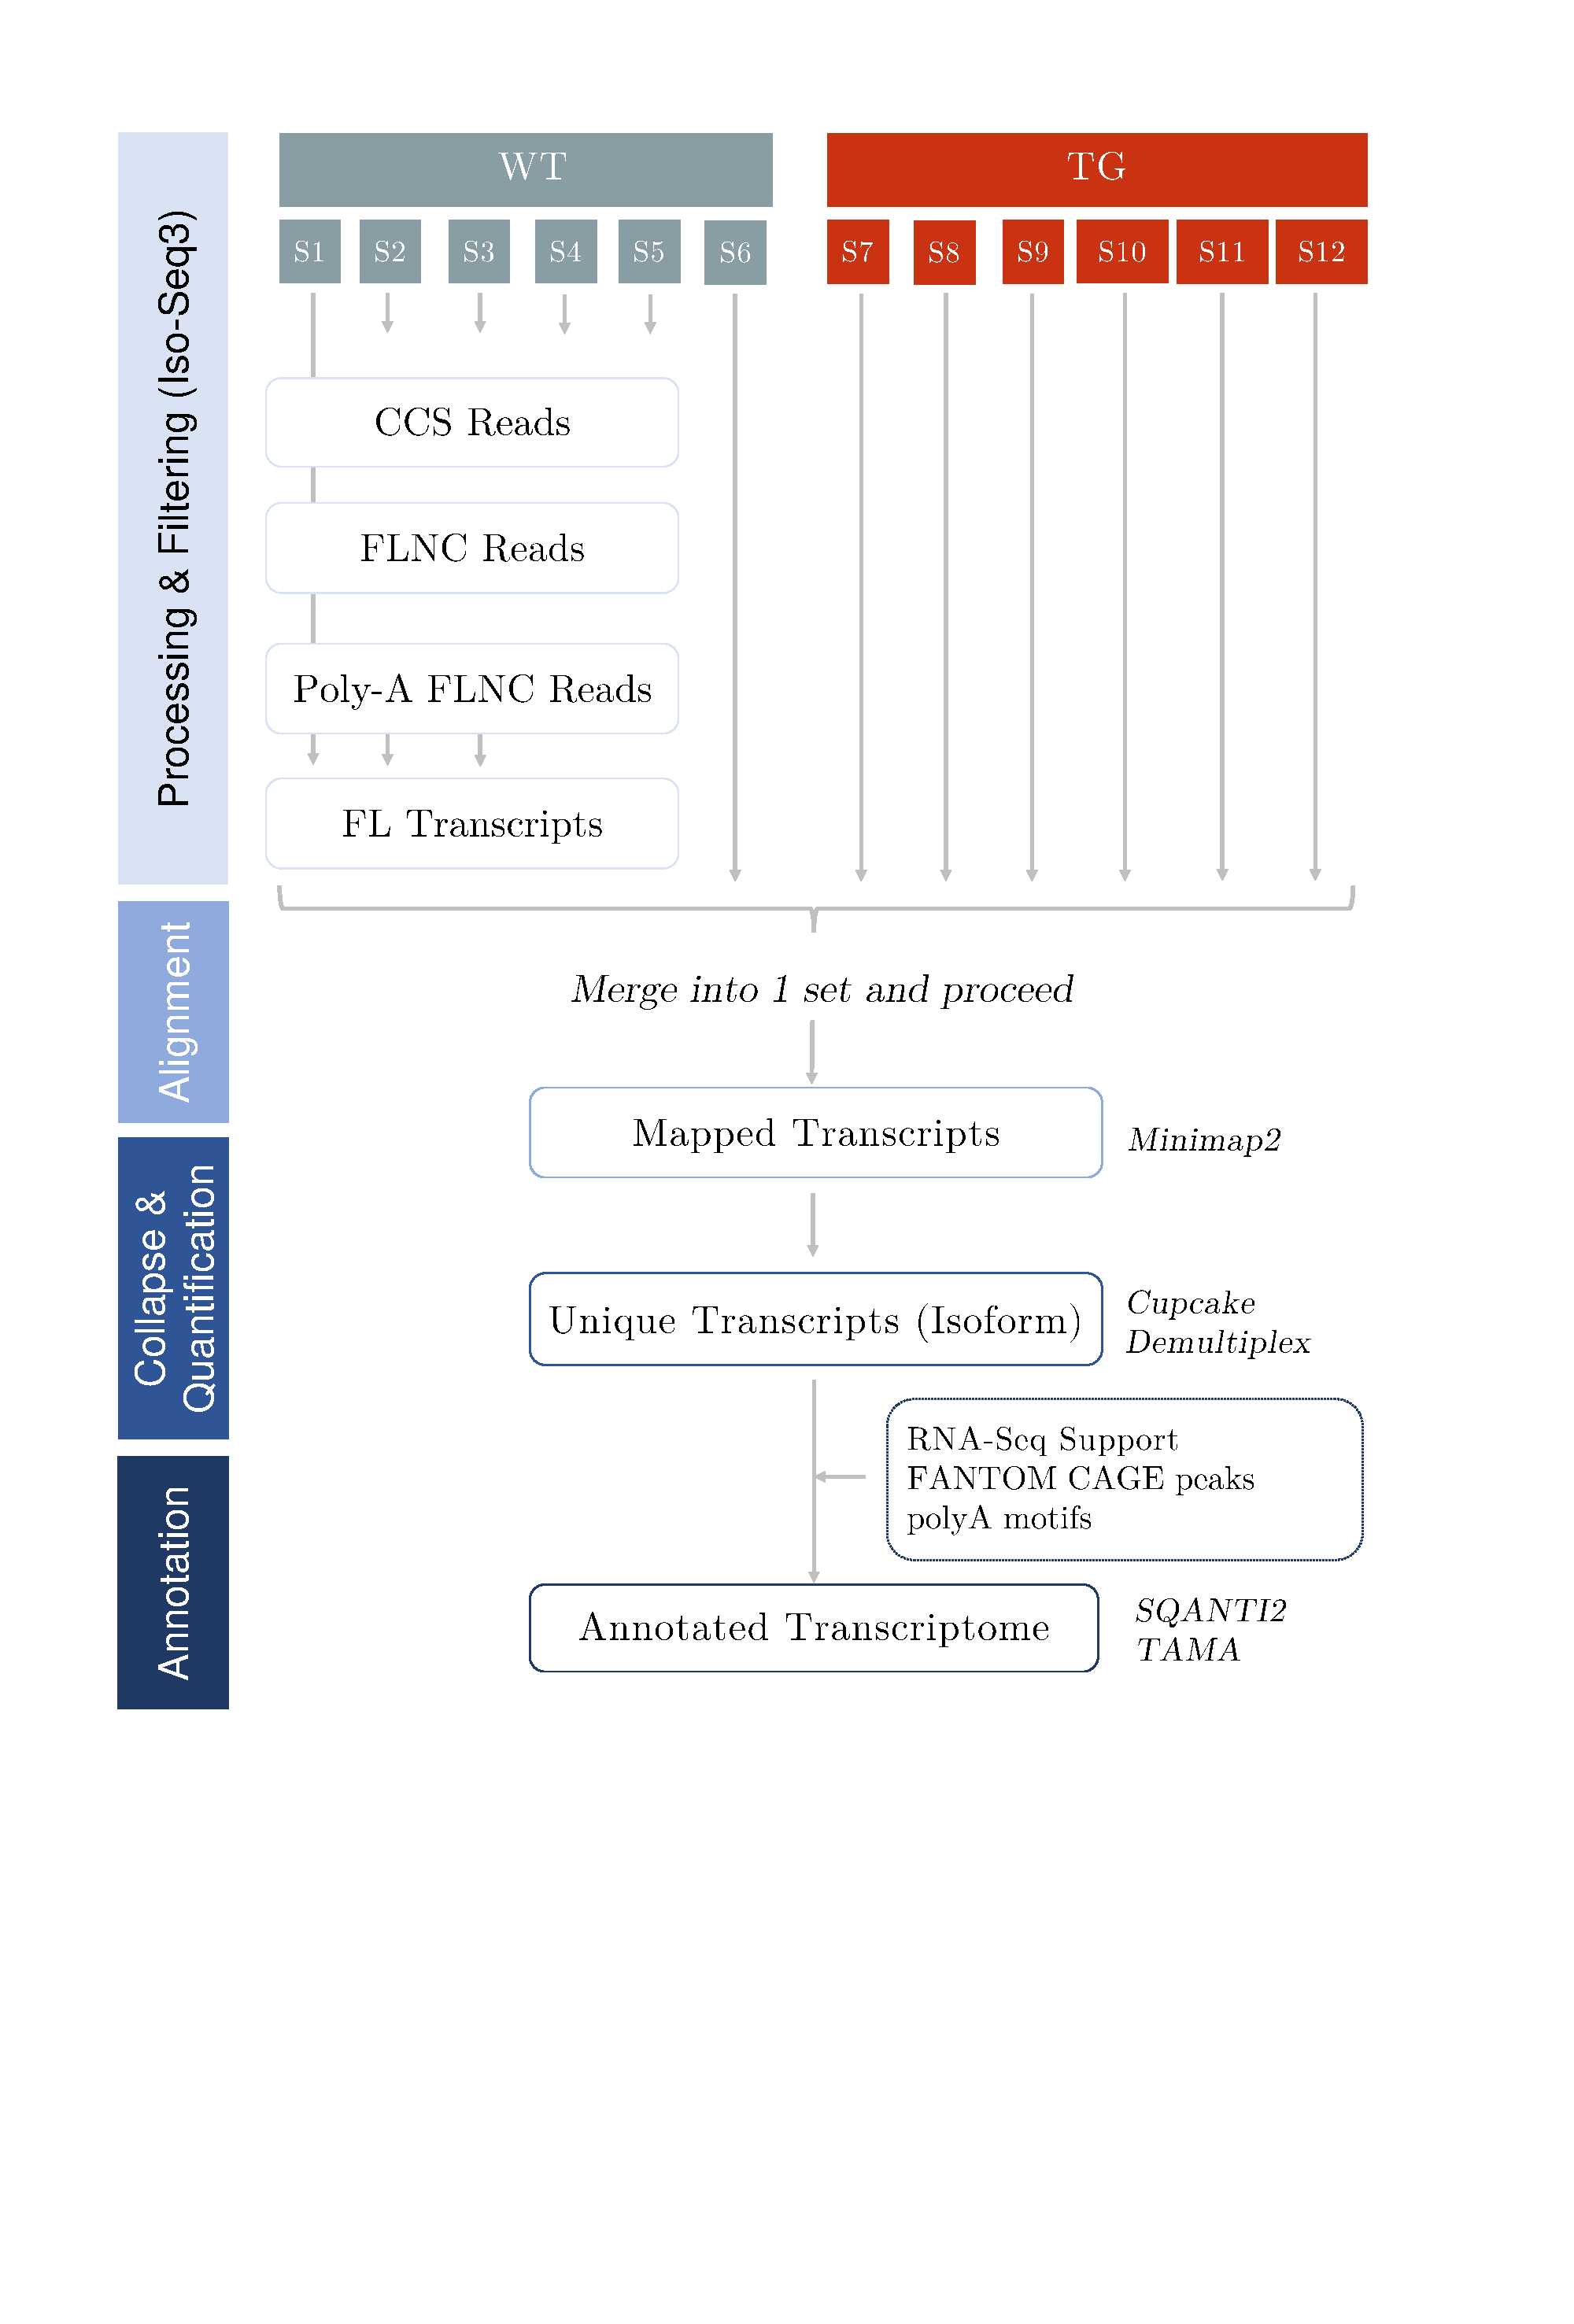
\includegraphics[page=1,trim={0 12cm 2cm 1cm},clip, scale = 0.45]{Figures/Pipeline.pdf}
	\captionsetup{width=0.95\textwidth}
	\caption[PacBio Iso-Seq Bioinformatics Pipeline for global transcriptome profiling]%
	{\textbf{PacBio Iso-Seq Bioinformatics Pipeline for global transcriptome profiling}: An overview of the analysis pipeline used to generate full-length transcript annotations in mouse entorhinal cortex samples (n = 12, WT = 6, TG = 6). Briefly, polymerase reads from PacBio Sequel for each dataset were processed using \textit{Iso-Seq 3.1.2} and Cupcake scripts to generate high quality, full-length isoforms, which were mapped to mouse reference genome using \textit{Minimap2}. \textit{SQANTI2} was used to fully annotate individual isoforms, with comparison to short-read RNA-Seq and reference annotations. Additional details are provided in \cref{section:isoseq_bioinformatics}. CCS - Circular Consensus Sequence, FLNC - Full-length non-chimeric, FL - Full-length}
	\label{fig:isoseq_whole_pipeline}
\end{figure}
 
\newpage
\section{Results}

\subsection{PacBio Iso-Seq run performance and sequencing metrics}
Following library preparation and SMRT sequencing, we generated a total of 371Gb (s.d = 4.35Gb, range = 22.5Gb - 38.7Gb) and 8,082,647 polymerase reads (s.d = 63,013 reads, range = 530,974 - 733,495 reads) (\cref{tab:isoseq_wholerun_result}). Following the Iso-Seq bioinformatics pipeline, raw reads were processed and clustered to unique consensus transcripts, which were then mapped to the genome and annotated. A total of 5.66M CCS reads (mean = 471K, s.d = 46.8K, range =  353K - 512K) and 4.55 FLNC reads were successfully generated (mean = 379K, s.d = 47.0K, range = 270K - 412K). Clustering of these reads yielded a total of 273K high-quality full-length transcripts (97\% of all FL transcripts, mean = 32.7K, s.d = 1.25K, range = 30.3K - 34.4K), and were mapped to 278K and 352 loci of the mouse reference (5K had multi-mapping) and ERCC annotations respectively. The majority of CCS reads were sized 2 - 3kb in length (mean length = 2.6kb), corresponding to the mean length of mRNA in the mouse reference genome. After filtering for 85\% alignment identity and 95\% length, 266K transcripts were retained. Rarefaction curves confirmed that the dataset approached saturation, indicating that our coverage of isoform diversity was representative of the true population of transcripts. 

\subsection{Widespread isoform diversity in the mouse cortex}
Following stringent quality-control, Iso-Seq reads mapped to 14,482 ‘annotated’ genes with expression patterns reflecting those expected for the cortex; using the Mouse Gene Atlas database, the 500 most abundantly-expressed genes were most significantly enriched for ‘cerebral cortex’ (odds ratio = 6.07, adjusted P = 6.8 x 10\textsuperscript{-17}). We identified 46,626 unique transcripts (mean length = 3.18kb, s.d = 1.68kb, range = 0.083 – 15.9kb), which were enriched near Cap Analysis Gene Expression (CAGE) peaks from the FANTOM5 dataset (median distance from CAGE peak = -1bp, 35,262 (75.6\%) transcripts located within 50bp of a CAGE peak), and were also located proximal to annotated transcription start sites and transcription termination sites. A significant proportion of isoforms (20,621, 45\%) were sized 2 - 4kb in length (median length = 2.96kb, mean length = 3.18kb, s.d = 1.68kb, range = 0.083 - 15.9kb) (\cref{fig:isoseq_whole_isoform_length_corr}\textbf{a}), corresponding to the mean length of mRNA mouse reference genome, with a wide range in the number of exons (1 - 89) observed per isoform (mean number of exons = 10.8). There was a wider range in the number of multi-exonic RNA isoforms identified per gene (1 - 86), with each gene associated with a median of 2 isoforms. Only 10\% (n = 4,641) of isoforms were detected across all the samples (\cref{fig:isoseq_whole_lowlyexp}\textbf{a}), with about half (47.8\%) detected in 2 - 3 samples with very low transcript expression (\cref{fig:isoseq_whole_lowlyexp}\textbf{b}). The number of detected isoforms was correlated with both gene length (corr = 0.25, P = 1.33 x 10-197;) and exon number (corr = 0.25, P = 4.02 x 10-193), with a stronger relationship observed amongst ‘highly-expressed’ genes.

\begin{figure}[!h]
	\begin{center}
		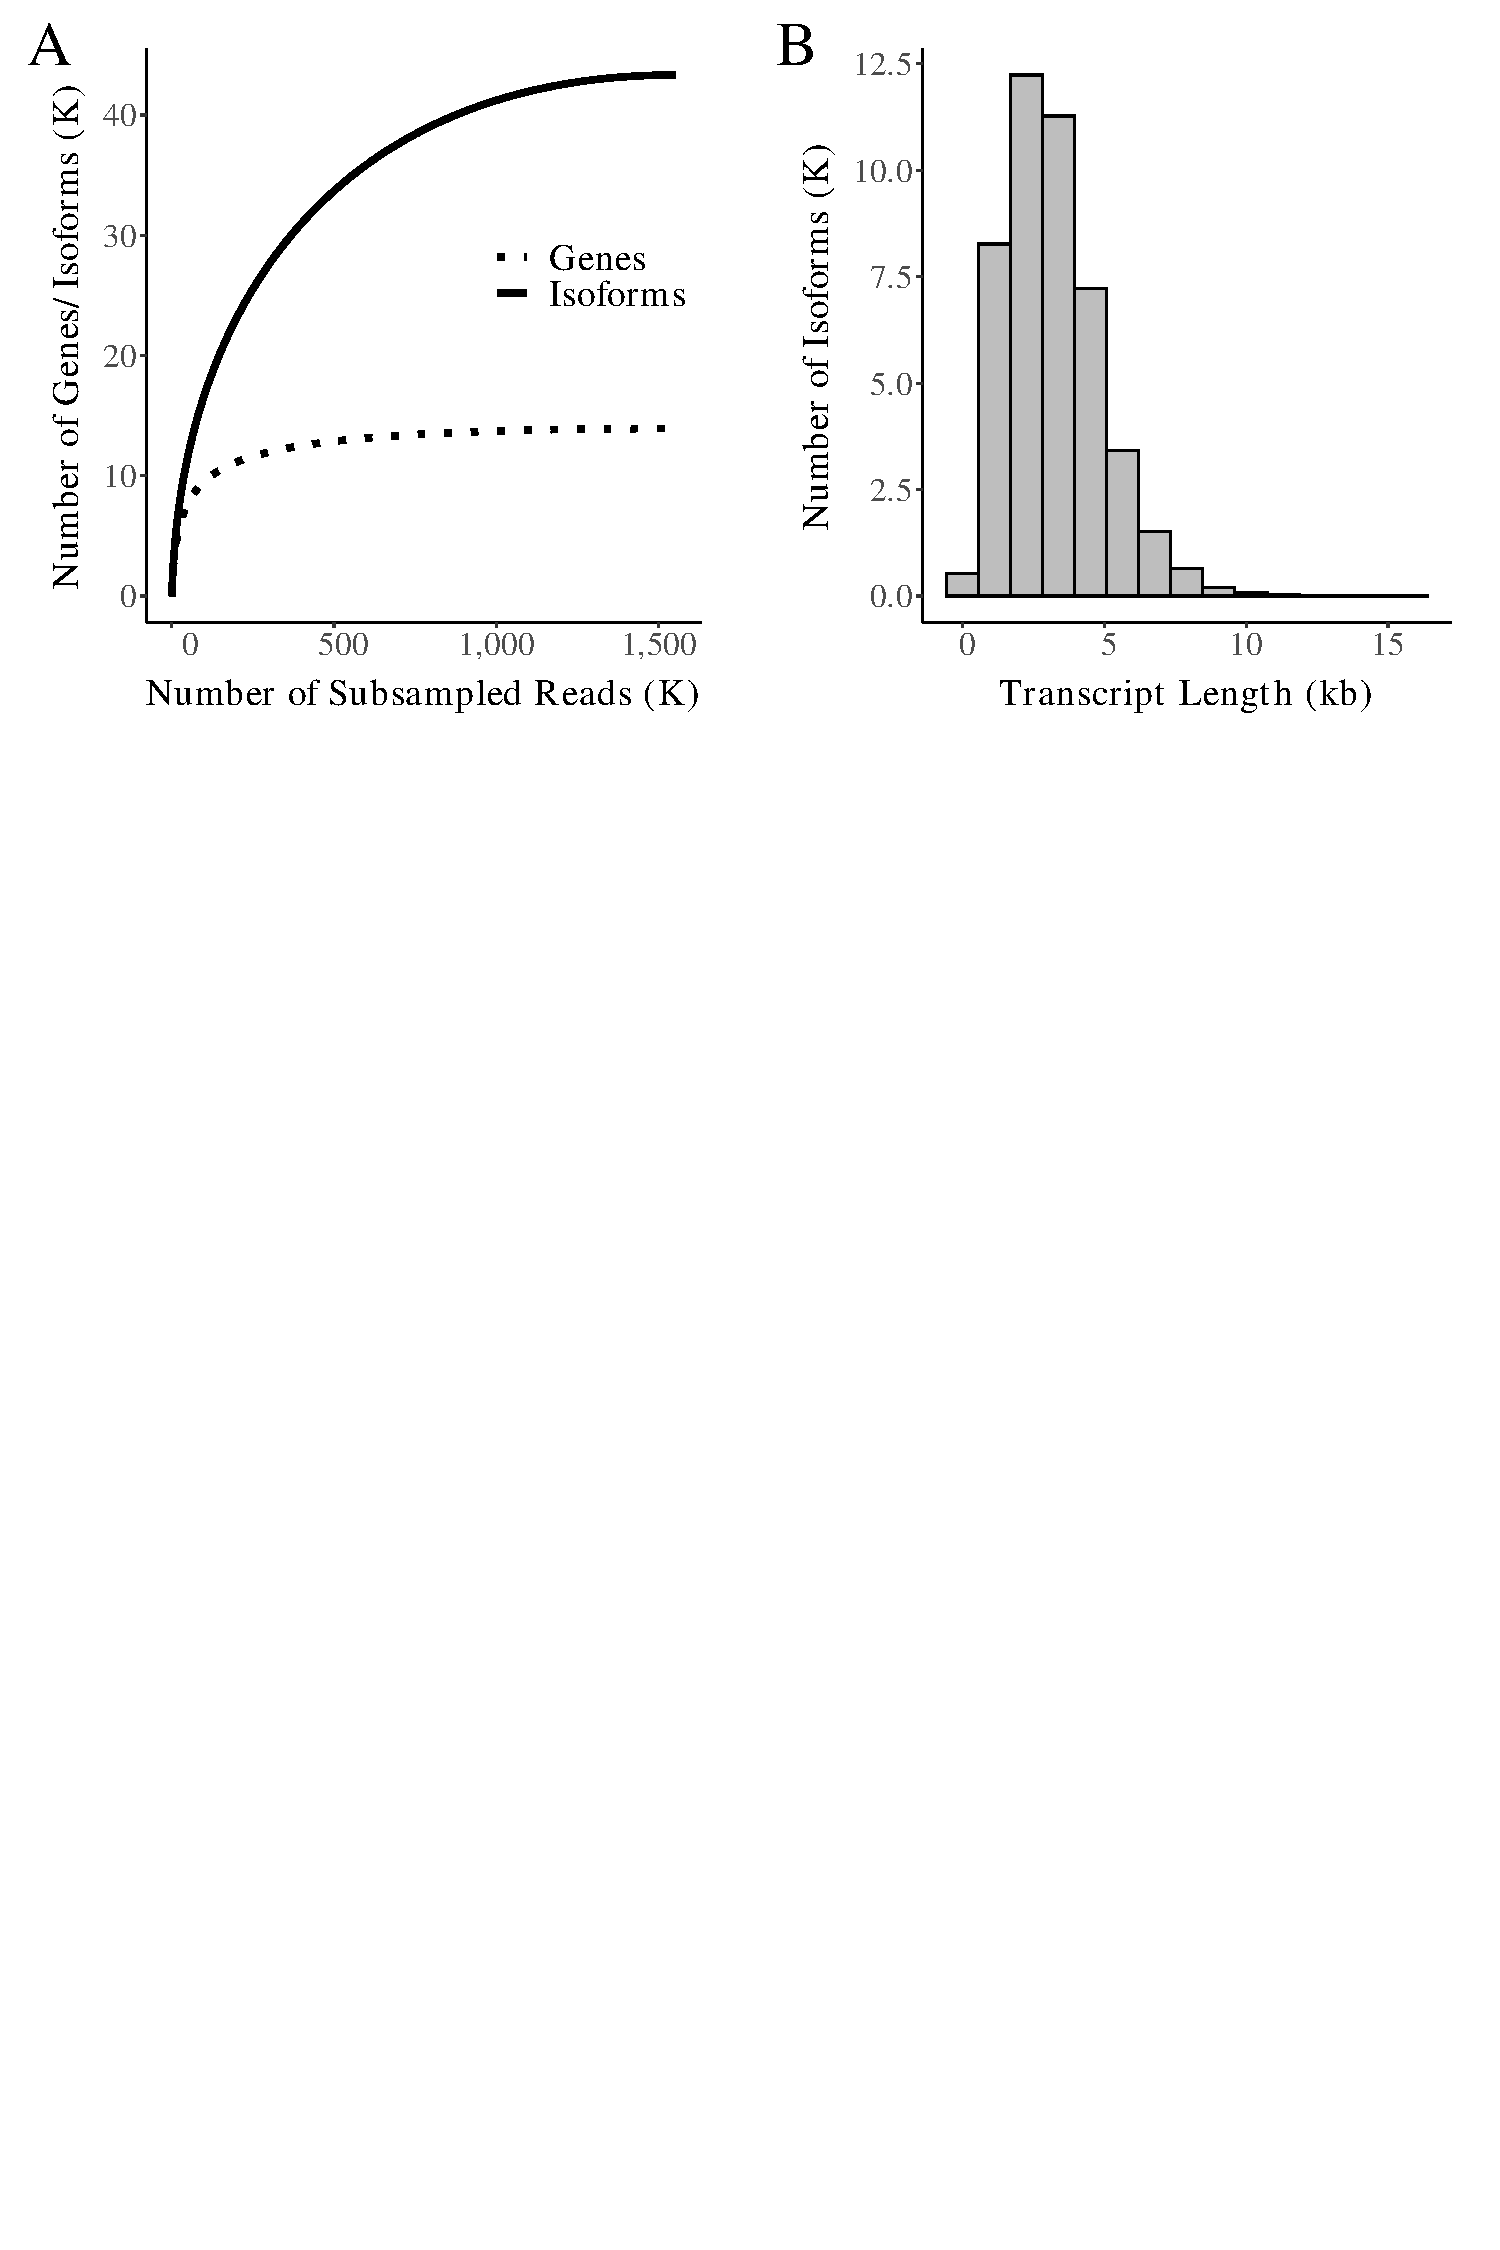
\includegraphics[page=1,trim={0 26cm 0 0},clip,scale = 0.55]{Figures/IsoSeqWholeTranscriptome.pdf}
	\end{center}
	\captionsetup{width=0.95\textwidth}
	\caption[Rarefaction Curves of Whole Transcriptome Iso-Seq Runs]%
	{\textbf{Rarefaction curve of Iso-Seq merged dataset indicated saturation and good coverage of genes and isoforms}:\textbf{a} The majority of isoforms have a length between 1 - 5kb.}
	\label{fig:isoseq_whole_rarefaction}
\end{figure}

\begin{figure}[!h]
	\begin{center}
		\includegraphics[page=3,trim={0 26cm 0 0},clip,scale = 0.55]{Figures/IsoSeqWholeTranscriptome.pdf}
	\end{center}
	\captionsetup{width=0.95\textwidth}
	\caption[Isoform diversity across Tg4510 samples and coverage of ERCC transcripts]%
	{\textbf{Highly-expressed isoforms are more likely to be sequenced across samples and accurately quantified}: Shown is \textbf{a)} the distribution of isoforms detected in the number of mouse samples, with a third detected in any two of the total 12 samples. However, \textbf{b)} quantification of these isoforms had very low expression (1-2 FL read), whereas those that were commonly detected across all 12 samples were very highly expressed. FL - Full Length}
	\label{fig:isoseq_whole_lowlyexp}
\end{figure}

\begin{landscape}
\begin{table}[]
	\captionsetup{width=1.5\textwidth}
	\caption[Run Yield Output from Whole Transcriptome Iso-Seq of Tg4510]%
	{Iso-Seq run yield for each sample of Tg4510 sequenced using Whole Transcriptome approach}
	\label{tab:isoseq_wholerun_result}
	\resizebox{1.5\textwidth}{!}{%
	\centering
	\begin{tabular}{@{}ccccccccccccccccccc@{}}
		\toprule
		\multirow{3}{*}{\begin{tabular}[c]{@{}c@{}}Sample   \\ ID\end{tabular}} &
		\multirow{3}{*}{\begin{tabular}[c]{@{}c@{}}Total \\ Bases \\ (GB)\end{tabular}} &
		\multirow{3}{*}{\begin{tabular}[c]{@{}c@{}}Pol\\ Reads \\ (K)\end{tabular}} &
		\multicolumn{6}{c}{Read   Length (kB)} &
		\multicolumn{3}{c}{Productivity} &
		\multicolumn{4}{c}{Control} &
		\multirow{3}{*}{\begin{tabular}[c]{@{}c@{}}Local \\ Base\\ Rate\end{tabular}} &
		\multicolumn{2}{c}{Template} \\ \cmidrule(lr){4-16} \cmidrule(l){18-19} 
		&
		&
		&
		\multicolumn{2}{c}{Polymerase} &
		\multicolumn{2}{c}{Subread} &
		\multicolumn{2}{c}{Insert} &
		\multirow{2}{*}{P0} &
		\multirow{2}{*}{P1} &
		\multirow{2}{*}{P2} &
		\multirow{2}{*}{\begin{tabular}[c]{@{}c@{}}Total   \\ Reads\end{tabular}} &
		\multirow{2}{*}{\begin{tabular}[c]{@{}c@{}}Length   \\ (Kb)\end{tabular}} &
		\multicolumn{2}{c}{Concordance} &
		&
		\multirow{2}{*}{\begin{tabular}[c]{@{}c@{}}Adapter \\ Dimer\end{tabular}} &
		\multirow{2}{*}{\begin{tabular}[c]{@{}c@{}}Short\\ Insert\end{tabular}} \\ \cmidrule(lr){4-9} \cmidrule(lr){15-16}
		&&&	Mean &	N50 & Mean & N50 &	Mean &	N50 &
		&&&&&
		Mean &	Mode &&&
		\\ \midrule
		Mouse 1 & 29.56 & 674 &	43.86 &	90.56 &	1.25 & 2.02 & 3.34 & 4.75 &
		\begin{tabular}[c]{@{}c@{}}10.55\% \\ (107K)\end{tabular} &
		\begin{tabular}[c]{@{}c@{}}67.42\% \\ (682K)\end{tabular} &
		\begin{tabular}[c]{@{}c@{}}22.73\% \\ (230K)\end{tabular} &
		7036 &	34.7 &	0.85 &	0.89 &	2.72 &	0.08 &	0.06 \\
		Mouse 2 & 31.1 & 566 & 54.89 & 101.22 &	1.26 &	1.78 & 2.86 & 3.66 &
		\begin{tabular}[c]{@{}c@{}}29.77\% \\ (300K)\end{tabular} &
		\begin{tabular}[c]{@{}c@{}}57.25\% \\ (577K)\end{tabular} &
		\begin{tabular}[c]{@{}c@{}}14.05\%\\ (142K)\end{tabular} &
		10707 &	44.6 &	0.87 &	0.89 &	3.05 &	0 &	0 \\
		Mouse 3 & 34.60 & 698 & 49.56 &	98.80 &	1.70 &	2.67 &	3.78 &	4.78 &
		\begin{tabular}[c]{@{}c@{}}16.1\% \\ (164K)\end{tabular} &
		\begin{tabular}[c]{@{}c@{}}69.2\%  \\ (704K)\end{tabular} &
		\begin{tabular}[c]{@{}c@{}}14.7\% \\ (150K)\end{tabular} &
		5951 &	40.5 &	0.85 &	0.89 &	2.78 &	0 &	0 \\
		Mouse 4 &	34.61 &	711 &	48.68 &	97.02 &	1.71 &	2.49 &	3.83 &	5.02 &
		\begin{tabular}[c]{@{}c@{}}14.22\% \\ (145K)\end{tabular} &
		\begin{tabular}[c]{@{}c@{}}70.49\%\\ (718K)\end{tabular} &
		\begin{tabular}[c]{@{}c@{}}15.28\%\\ (156K)\end{tabular} &
		6762 &	38.4 &	0.85 &	0.87 &	2.671 &	0.01 &	0.01 \\
		Mouse 5 &	38.74 & 675 &	57.37 &	112.63 &	1.87 &	2.87 &	3.90 &	4.79 &
		\begin{tabular}[c]{@{}c@{}}17.41\% \\ (176K )\end{tabular} &
		\begin{tabular}[c]{@{}c@{}}68.08\% \\ (686K)\end{tabular} &
		\begin{tabular}[c]{@{}c@{}}15.575 \\ (157K)\end{tabular} &
		10647 &	44.2 &	0.86 &	0.89 &	2.96 &	0.01 &	0 \\
		Mouse 6 &	30.45 &	661 &	46.08 &	91.63 &	2.23 &	2.75 &	3.95 &	4.73 &
		\begin{tabular}[c]{@{}c@{}}16.6\% \\ (169K)\end{tabular} &
		\begin{tabular}[c]{@{}c@{}}65.9\% \\ (671K)\end{tabular} &
		\begin{tabular}[c]{@{}c@{}}17.5\% \\ (179K)\end{tabular} &
		10301 &	38.7 &	0.85 &	0.87 &	2.79 &	0.01 &	0.01 \\
		Mouse 7 &	22.53 &	531 &	42.42 &	85.33 &	2.61 &	3.15 &	3.44 &	4.08 &
		\begin{tabular}[c]{@{}c@{}}41.8\% \\ (426K)\end{tabular} &
		\begin{tabular}[c]{@{}c@{}}52.6\% \\ (536K)\end{tabular} &
		\begin{tabular}[c]{@{}c@{}}5.5\% \\ (56.4K)\end{tabular} &
		5415 &	49.8 & 0.86 &	0.85 &	2.05 &	0 &	0 \\
		Mouse 8 &	31.25 &	731 &	42.77 &	89.37 &	1.49 &	2.35 &	3.61 &	4.88 &
		\begin{tabular}[c]{@{}c@{}}9.37\% \\ (94.5K)\end{tabular} &
		\begin{tabular}[c]{@{}c@{}}73.33\% \\ (740K)\end{tabular} &
		\begin{tabular}[c]{@{}c@{}}18.19\% \\ (184K)\end{tabular} &
		8908 &	35.0 &	0.85 &	0.89 &	2.56 &	0.06 &	0.04 \\
		Mouse 9 &	33.16 &	715 &	46.36 &	92.52 &	2.00 &	2.93 &	3.98 &	4.95 &
		\begin{tabular}[c]{@{}c@{}}11.51\%\\ (117K)\end{tabular} &
		\begin{tabular}[c]{@{}c@{}}70.91\% \\ (722K)\end{tabular} &
		\begin{tabular}[c]{@{}c@{}}17.58\% \\ (18.0K)\end{tabular} &
		6855 &	38.0 &	0.85 &	0.87 &	2.6 &	0.01 &	0.01 \\
		Mouse 10 &	24.52 &	733 &	33.43 &		70.75 &	2.56 &	3.29 &	3.71 &	4.75 &
		\begin{tabular}[c]{@{}c@{}}15.9\% \\ (162K)\end{tabular} &
		\begin{tabular}[c]{@{}c@{}}72.1\% \\ (735K)\end{tabular} &
		\begin{tabular}[c]{@{}c@{}}12.0\% \\ (122K)\end{tabular} &
		1668 & 44.2 &	0.85 &	0.85 &	1.99 &	0.00 &	0.01 \\
		Mouse 11 &	30.41 &	683 &	44.55 &	90.04 &	1.44 &	2.04 &	3.28 &	4.40 &
		\begin{tabular}[c]{@{}c@{}}11.98\%\\ (121K)\end{tabular} &
		\begin{tabular}[c]{@{}c@{}}68.45\% \\ (692K)\end{tabular} &
		\begin{tabular}[c]{@{}c@{}}20.35\% \\ (206K)\end{tabular} &
		7881 &	36.5 &	0.86 &	0.89 &	2.85 &	0.11 &	0.07 \\
		Mouse 12 &	30.28 &	704 &	42.99 &	89.16 &	1.35 &	2.02 &	3.27 &	4.38 &
		\begin{tabular}[c]{@{}c@{}}7.02\%\\ (71.1K)\end{tabular} &
		\begin{tabular}[c]{@{}c@{}}70.18\% \\ (710K)\end{tabular} &
		\begin{tabular}[c]{@{}c@{}}23.39\% \\ (237K)\end{tabular} &
		6019 &	35.2 &	0.85 &	0.89 &	2.57 &	0.01 &	0.01 \\ \bottomrule
	\end{tabular}%
}
\end{table}
\end{landscape}

\subsection{Detection of many novel isoforms with novel junctions}
\label{sec:whole_novelIso}
Amongst full-length transcripts annotated to known genes, 50\% (n = 23,096) were novel and not present in existing annotation databases (\cref{tab:sqanti_output_whole}). Compared to known isoforms, these novel isoforms were less abundant (Mann-Whitney-Wilcoxon test, W = 3.66 x 108, P < 2.23 x 10\textsuperscript{-308} \cref{fig:isoseq_whole_novel_known_iso_corr}\textbf{a,b}) and longer (W = 2.37 x10\textsuperscript{8}, P = 2.13 x 10\textsuperscript{-42}, \cref{fig:isoseq_whole_novel_known_iso_corr}\textbf{c,d}) and had more exons (W = 1.94 x 10\textsuperscript{8}, P < 2.23 x 10\textsuperscript{-308}, \cref{fig:isoseq_whole_novel_known_iso_corr}\textbf{e,f}), suggesting that they would have been harder to detect using RNA-Seq due to the difficulty in assembling transcripts with limited read coverage. These novel isoforms were also more likely to be associated with novel transcription start sites (1,454 novel vs 1,154 known isoforms at least 1kb away from known TSS, Fisher's Test: P = 6.16 x 10\textsuperscript{-12}, odds ratio = 1.32) and termination sites (21,506 novel vs 21,434 annotated isoforms less than 1kb away from known TTS). Assessing the reliability of novel isoforms against known, there was no difference in the number supported within 50bp of CAGE peak (17,252 (75.4\%) novel vs 17,842 (75.8\%) known isoforms, Fisher's Test: P = 0.31, odds ratio = 0.978). While there was less RNA-Seq support for novel isoforms ( 8.95TPM mean RNA-Seq expression for known vs 1.99TPM novel isoforms; two-tailed unpaired t-test: t(46401) = 14.8, P = 1.37 x 10\textsuperscript{-49}), this is a likely reflection of the relatively lower expression of novel isoforms and RNA-Seq's lack of power to detect them.

\vspace{1cm}
\begin{table}[!h]
	\caption[Gene and Isoform classification from Whole Transcriptome Iso-Seq of Tg4510]%
	{Classification of annotated and novel genes and isoforms were based from SQANTI2, and from the merging of 12 samples. FSM - Full Splice Match, ISM - Incomplete Splice Match, NIC - Novel In Catalogue, NNC - Novel Not in Catalogue }
	\label{tab:sqanti_output_whole}
	\begin{tabularx}{1\textwidth}{lcl}
		\toprule
		Description              & \multicolumn{1}{l}{Number} & Isoform Definition               \\ \midrule
		Number of Genes    & 14684                      &                                  \\
		Number of Isoforms & 46626                      &                                  \\
		Annotated Genes          & 14482 (98.62\%)            &                                  \\
		\hspace{3mm}Annotated Isoforms       & 23530 (50.47\%)            &                                  \\
		\hspace{6mm}FSM          & 19803 (42.47\%) & exact alignment as reference  \\
		\hspace{6mm}ISM  & 3727 (7.99\%)   & exact alignment as reference but fewer 5’ exons       \\
		\hspace{3mm}Novel Isoforms           & 23096 (49.53\%)            &                                  \\
		\hspace{6mm}NIC      & 13763 (29.52\%) & a combination of known donor/acceptor sites                    \\
		\hspace{6mm}NNC   & 8751 (18.77\%)  & at least one novel donor/acceptor site    \\
		\hspace{6mm}Fusion                   & 297 (0.64\%)               &                                  \\
		\hspace{6mm}Genic Genomic            & 62 (0.13\%)                & overlaps with introns and exons  \\
		Novel Genes              & 202 (1.38\%)               &                                  \\
		\hspace{6mm}Intergenic               & 104 (0.22\%)               & located in the intergenic region \\
		\hspace{6mm}Antisense                     & 119 (0.26\%)    & opposite-strand orientation to known gene           \\ \bottomrule
	\end{tabularx}
\end{table}

\begin{figure}[!htp]
	\begin{center}
		\includegraphics[page=4,scale = 0.55]{Figures/IsoSeqWholeTranscriptome.pdf}
	\end{center}
	\captionsetup{width=0.95\textwidth}
	\caption[Comparison of Known and Novel Isoforms from Iso-Seq Whole Transcriptome runs]%
	{\textbf{Novel isoforms were less expressed, longer and had more exons than known isoforms}: Shown is the \textbf{a)} Iso-Seq transcript expression, the \textbf{c)} transcript length, and the \textbf{e)} the number of exons of novel and known isoforms. The known and novel isoforms can be further subdivided and classified, with the \textbf{b)} Iso-Seq expression \textbf{d)} transcript length and \textbf{f)} number of exons for each category. According to SQANTI, known isoforms are subdivided into FSM and ISM, and novel isoforms are subdivided into NIC, NNC, and fusion. FSM – Full Splice Match, ISM – Incomplete Splice Match, NIC – Novel In Catalogue, NNC – Novel Not in Catalogue.}   
	\label{fig:isoseq_whole_novel_known_iso_corr}
\end{figure}


\newpage
\subsection{Comparisons with RNA-Seq confirm Iso-Seq sensitivity} 
\label{sec: whole_isoseqvsrnaseq}
Although Iso-Seq is accurate at characterizing RNA diversity\cite{Wang2019}, its sensitivity for quantifying gene expression has not been systematically explored. Generating highly-parallel RNA-Seq data on the same samples, we find a strong correlation between gene-level expression quantified using the two methods in both datasets. To further assess the quantitative accuracy of Iso-Seq, we included ERCC spike-in control molecules. Among the detected ERCC transcripts (n = 57, 62\%) we found a near-perfect correlation between full-length Iso-Seq reads and the actual amount of control used (corr = 0.98, P = 1.42 x 10\textsuperscript{-41}), highlighting the power of Iso-Seq to accurately quantify the abundance of highly-expressed transcripts. The vast majority of unique splice junctions identified in our Iso-Seq data were supported by RNA-Seq (n = 152,872 (98.1\%) junctions). For transcripts that could be recapitulated in the matched RNA-Seq data, there was a significant correlation between transcript expression levels quantified using both sequencing approaches (n = 41,488 transcripts, corr = 0.48, P < 2.23 x 10\textsuperscript{-308}) further highlighting that transcript abundance can be reliably quantified using Iso-Seq. 

Using our Iso-Seq data as a scaffold, we generated a reference-guided transcriptome assembly from our mouse cortex RNA-Seq data using Stringtie\cite{Pertea2015}. Many of the isoforms reconstructed from RNA-Seq reads appeared to represent incomplete fragments of full-length transcripts identified in Iso-Seq. Overall, isoforms assembled using RNA-Seq reads had a significantly shorter mean length (RNA-Seq: 2.31kb vs Iso-Seq: 3.18kb, t = 71.9, P < 2.2 x 10\textsuperscript{-16}), lower average number of exons (RNA-Seq: 7.30 vs Iso-Seq: 10.8 , t = 76.7, P < 2.2 x 10\textsuperscript{-16}) and were less likely to be located within a CAGE peak (RNA-Seq: 34.0\% vs Iso-Seq: 71.9\%, Fisher’s Exact Test = P < 2.2 x 10-16, odds ratio = 4.97). Importantly, more than 50\% of isoforms robustly detected using Iso-Seq could not be readily recapitulated using standard RNA-Seq, highlighting the advantage of long-read sequencing for characterizing isoform diversity.%Finally, a large proportion of novel transcripts identified using Iso-Seq (n = 6,417 (53.78\%)) were also detected with ONT nanopore sequencing (40.7 million reads) from a subset of samples.  

\begin{figure}[htp]
	\begin{center}
		\includegraphics[page=3,trim={0 25cm 0 0},clip,scale = 0.55]{Figures/IsoSeqWholeTranscriptome.pdf}
	\end{center}
	\captionsetup{width=0.95\textwidth}
	\caption[Detection of ERCC standards in Whole Transcriptome Iso-Seq]%
	{\textbf{Over 60\% of ERCC were detected with highly accurate quantification} \textbf{a} Highly-concentrated ERCC were detected as single molecules, as expected, and \textbf{b} the number of full-length reads associated for each detected ERCC was highly correlated to known amount. FL - Full Length}
	\label{fig:isoseq_whole_ercc}
\end{figure}


\begin{figure}[htp]
	\begin{center}
		\includegraphics[page=9,trim={0 13cm 0 0},scale = 0.55]{Figures/IsoSeqWholeTranscriptome.pdf}
	\end{center}
	\captionsetup{width=0.95\textwidth}
	\caption[RNA-Seq defined transcriptome]%
	{\textbf{Iso-Seq identified more isoforms per gene, that were longer with more exons, and with a greater proportion of isoforms with CAGE peak}: A reference-guided transcriptome using only RNA-Seq data (RNA-Seq defined transcriptome) was generated. \textbf{a)} RNA-Seq defined transcriptome identified more isoforms, as expected given the significantly higher sequencing depth. However, \textbf{b)} the isoform diversity was smaller than that from Iso-Seq defined transcriptome with the majority of genes associated with only one isoform. \textbf{c)} Isoforms identified from the RNA-Seq defined transcriptome were also more likely to be shorter and \textbf{d} contain fewer exons. \textbf{e)} Highlighting the power of Iso-Seq to identify true full-length isoforms in comparison to RNA-Seq, a significantly larger proportion of isoforms from Iso-Seq data were found within 50bp of a CAGE peak. \textbf{f} Approximately half of the isoforms identified using Iso-Seq were novel (NIC, NNC), which were not recapitulated using RNA-Seq. FSM - Full Splice Match, ISM - Incomplete Splice Match, NIC - Novel In Catalogue, NNC - Novel Not in Catalogue.}   
	\label{fig:isoseq_whole_rnaseqvsisoseq}
\end{figure}

\subsection{Detection of transcripts with fusion events across genes}
Transcriptional read-through between two or more adjacent genes can produce ‘fusion transcripts’ that represent an important class of mutation in several types of cancer\cite{McCartney2019}. Although fusion events are thought to be rare\cite{Akiva2006a}, we found evidence of fusion transcripts (n = 297 fusion transcripts (0.64\% of all transcripts) associated with 218 genes (1.48\% of total genes), \cref{fig:isoseq_whole_novelfusion}\textbf{a,b}). A number of these genes were associated with more than one fusion transcript (n = 53 genes (24.3\% of fusion genes)), with the vast majority supported by RNA-Seq data (n = 282 (95\%) transcripts). 

\subsection{Iso-Seq identifies novel cortex-expressed genes}
\label{sec:whole_novelgenes}
Although the vast majority of isoforms were annotated to known genes, a small number represent expression from potentially novel genes (n = 189 genes).  These novel genes were either intergenic or antisense to existing annotated genes, and were all multi-exonic (mean length = 1.75kb, s.d = 1.21kb, range = 0.098 - 6.86kb, mean number of exons = 2.5). More than half of the transcripts from these novel genes were predicted to be non-coding (n = 143 (64.1\%) novel-gene transcripts), were generally shorter and less abundant than transcripts of annotated genes (length: W = 7.79 x 10\textsuperscript{6}, P = 5.22 x 10\textsuperscript{-45}; expression: W = 2.29x 10\textsuperscript{6}, P = 1.5 x 10\textsuperscript{-73}). Around a quarter of the novel-gene transcripts were enriched near CAGE peaks (n = 58 (26.0\%)) with over half were antisense transcripts to known genes (n = 119 transcripts (53.4\%) mapping to 97 novel genes). The majority of these antisense novel genes were found within an annotated gene (n = 95 (97.9\% of antisense novel genes)), with a relatively large proportion of these sharing exonic regions (exon-exon overlap, n = 72 (74.2\%)) reflecting sense-antisense (SAS) pairs. Finally, there were several striking examples of antisense novel genes overlapping two known genes (\cref{fig:isoseq_whole_novelfusion}\textbf{c}). 

\begin{landscape}
	\begin{figure}[htp]
		\begin{center}
			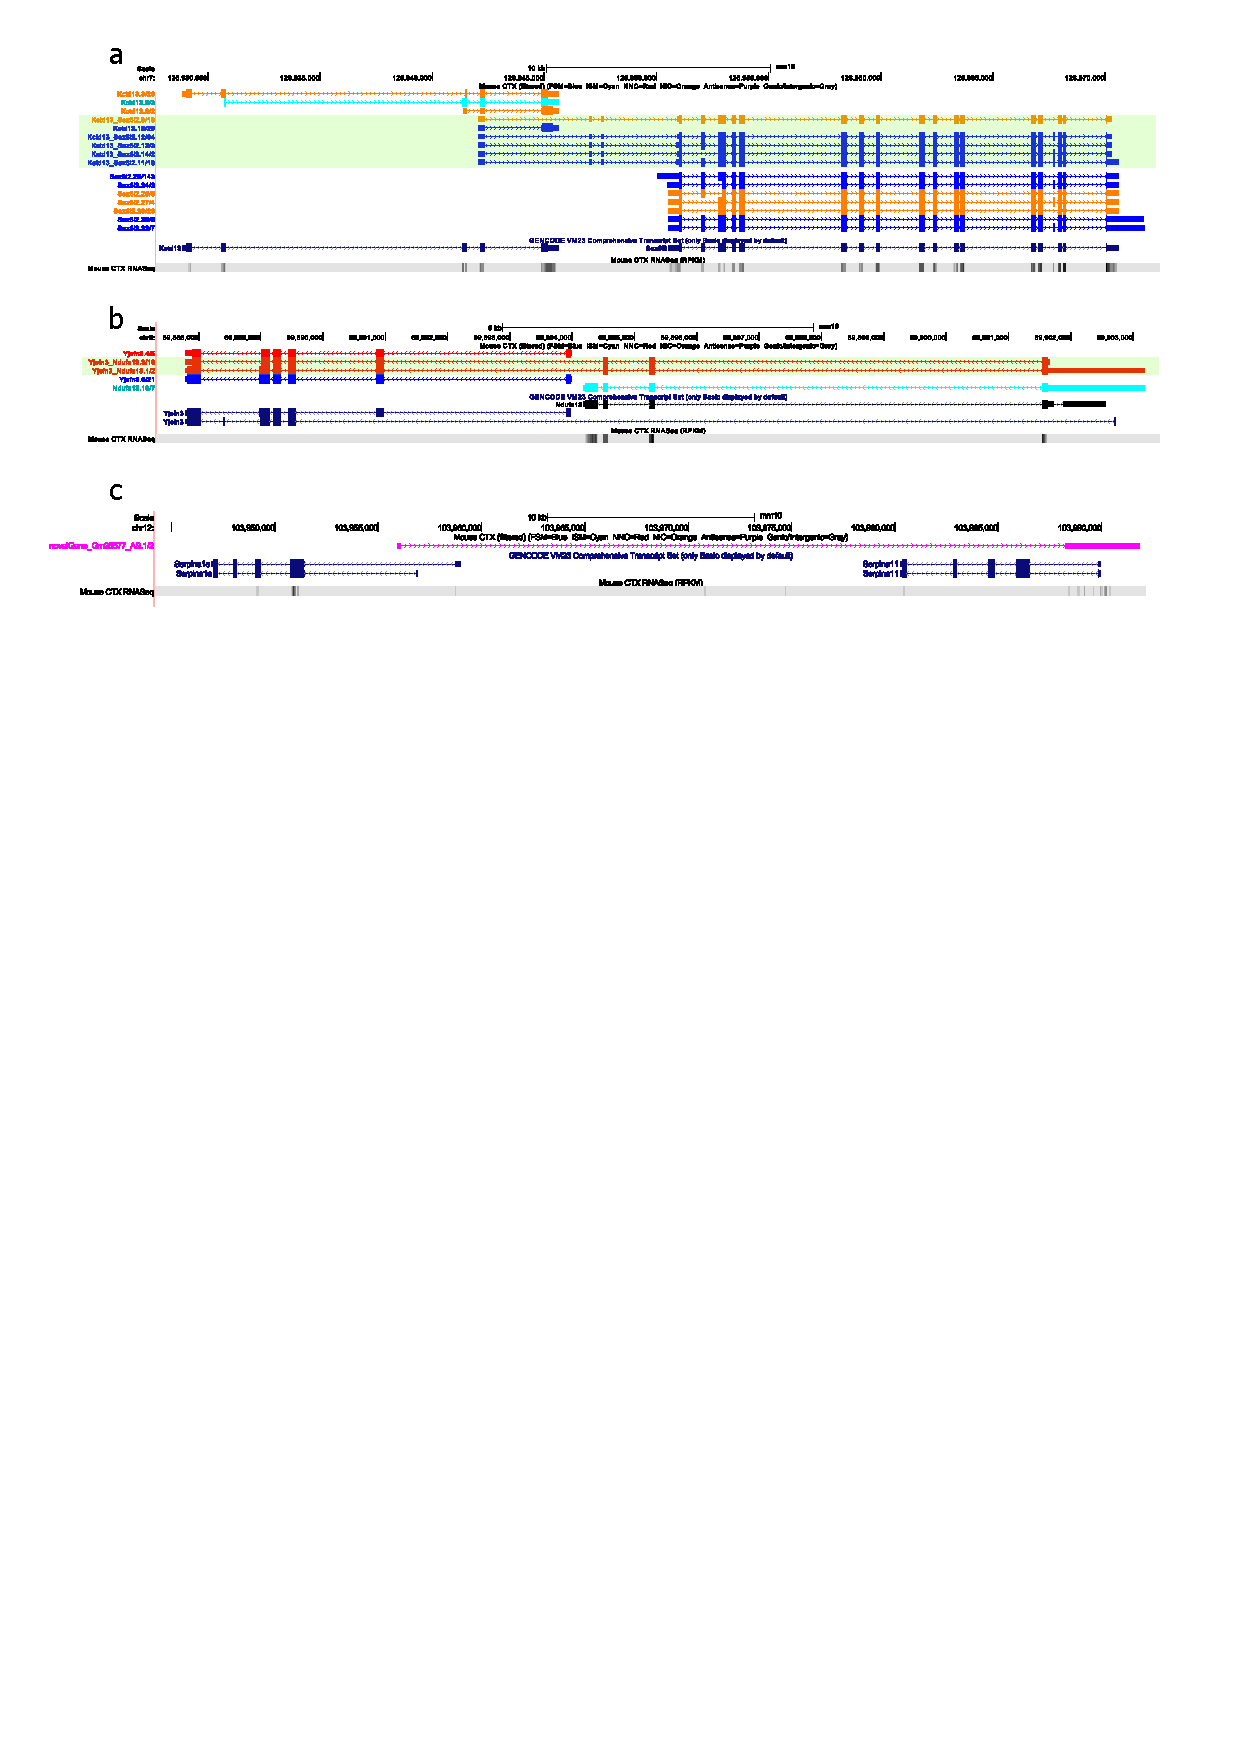
\includegraphics[page=1,trim={0 20cm 0 0},scale = 1.2]{Figures/FusionNovelGenes.pdf}
		\end{center}
		\vspace{1cm}
		\captionsetup{width=1.5\textwidth}
		\caption[Iso-Seq identifies fusion transcripts and novel genes in Mouse cortex]%
		{\textbf{Examples of fusion transcripts and novel genes identified in Mouse cortex}: \textbf{a)}Five read-through "fusion" transcripts incorporating exons from \textit{Kctd13} (SZ-associated) and \textit{Sez6I2} (SZ-associated). \textbf{b)} Two read-through "fusion" transcripts incorporating exons from \textit{Yjefn3} and \textit{Ndufa13} (SZ-associated). \textbf{c)} An example of a novel antisense transcript spanning \textit{Serpina1e} and \textit{Serpina11} in the mouse cortex. Transcripts are coloured based on \textit{SQANTI2} classification categories (blue = FSM, cyan = ISM, red = NNC, orange = NIC). Fusion transcripts are boxed in green. SZ - Schizophrenia.}   
		\label{fig:isoseq_whole_novelfusion}
	\end{figure}
\end{landscape}


\subsection{Many transcripts map to long non-coding RNA genes}
Although the majority of transcripts (93.6\%, 43,450) were classified as protein-coding by the presence of an ORF, a relatively large number of transcripts were annotated as encoding long non-coding RNA (lncRNA) (n = 1,141 transcripts associated with 734 genes). These lncRNA transcripts were shorter than non-lncRNA transcripts (mean length of lncRNA transcripts = 2.22kb, s.d =1.36kb, range = 0.148 - 8.49kb; mean length of non-lncRNA transcripts = 3.21kb, s.d = 1.68kb, range = 0.083 - 15.9kb; W = 3.52 x 10\textsuperscript{7}, P = 8.24 x 10\textsuperscript{-98}, \cref{fig:isoseq_whole_lncRNA}\textbf{a}), and contained fewer exons\cite{Statello2020} (W = 4.56 x 10\textsuperscript{7}, P < 2.23 x 10\textsuperscript{-308}, \cref{fig:isoseq_whole_lncRNA}\textbf{b}) with a dramatic enrichment of mono-exonic molecules\cite{Kuo2017} (n = 273 (23.9\%)) compared to non-lncRNA transcripts (mouse: n = 914 (2.02\%)). They were also characterised by lower transcript expression than non-lncRNA transcripts\cite{Statello2020, Liu2016a} (human: W = 2.27 x 10\textsuperscript{7}, P = 9.44 x 10\textsuperscript{-35}; mouse: W = 3.16 x 10\textsuperscript{7}, P = 5.67 x 10\textsuperscript{-40}, \cref{fig:isoseq_whole_lncRNA}\textbf{c}), with fewer isoforms identified per lncRNA gene compared to non-lncRNA genes (mean n = 1.55 vs 3.29, W = 7.40 x 10\textsuperscript{6}, P = 5.76 x 10\textsuperscript{-107}, \cref{fig:isoseq_whole_lncRNA}\textbf{e}). A small proportion of these annotated lncRNA transcripts contained a putative ORF (n = 153 (13.4\%), \cref{fig:isoseq_whole_lncRNA}\textbf{d}) supporting recent observations that some lncRNA have potential protein coding capacity\cite{Kageyama2011}, although the majority of such ORFs are unlikely to code for proteins\cite{Guttman2013}; of note, these ORFs were shorter than those identified in non-lncRNA transcripts (mean length = 139bp vs 519bp, W = 1.75 x 10\textsuperscript{7}, P = 8.33 x 10\textsuperscript{-195}). 

\begin{figure}[htp]
	\begin{center}
		\includegraphics[page=7,trim={0 1cm 0 0},scale = 0.55]{Figures/IsoSeqWholeTranscriptome.pdf}
	\end{center}
	\captionsetup{width=0.95\textwidth}
	\caption[Characterisation of LncRNA in Whole Transcriptome runs]%
	{\textbf{LncRNA isoforms were more lowly expressed and typically longer than non-lncRNA transcripts, despite containing fewer exons}: Shown is the distribution of the \textbf{a)} transcript length, \textbf{b)} number of exons, \textbf{c)} transcript expression, \textbf{d)} ORF length and the \textbf{e)} diversity of isoforms annotated to lncRNA and non-lncRNA.lncRNA – long non-coding RNA}
	\label{fig:isoseq_whole_lncRNA}
\end{figure}

\subsection{AS events heavily contribute to isoform diversity}
In total, 40,249 alternative splicing events were identified in known genes with AF (alternative TSS variation) and SE being the most prevalent (AF: 12,853, 31.9\%; SE: 8,686, 21.6\%, \cref{fig:isoseq_whole_As_events}\textbf{a}). Splicing events and frequency were also compared between known and novel isoforms. Except for AF and AL, all the other different splicing events, and in particularly intron retention, were more likely to be observed in novel isoforms. This highlights the power of Iso-Seq to recapitulate the usage of complex splicing events (Fisher's one-tailed Test, A3: P = 7.78 x 10 \textsuperscript{–14}, odds ratio = 1.34; A5: P = 1.21 x 10\textsuperscript{–13}, odds ratio = 1.45, IR: P < 2.23 x 10\textsuperscript{–16}, odds ratio = 4.92; MX: P = 4.18 x 10\textsuperscript{–11}, odds ratio = 1.81; SE: P < 2.23 x 10\textsuperscript{–16}, odds ratio = 1.57, \cref{fig:isoseq_whole_As_events}\textbf{a}), which would have otherwise been underestimated using RNA-Seq data. For the majority of genes characterised by splicing, only one or two AS events were observed (n = 10,708, 81.8\% of AS genes, \cref{fig:isoseq_whole_As_events}\textbf{b}), suggesting that AS events were often mutually independent. 

\vspace{1cm}
\begin{figure}[!h]
	\begin{center}
		\includegraphics[page=5,trim={0 26cm 0 0},clip,scale = 0.55]{Figures/IsoSeqWholeTranscriptome.pdf}
	\end{center}
	\captionsetup{width=0.95\textwidth}
	\caption[Number of Alternative Splicing Events in Whole Transcriptome Iso-Seq]%
	{\textbf{Alternative first is the most prevalent AS event, and novel isoforms are more likely to be characterised with complex AS events}: \textbf{a)} Proportion of AS events in annotated genes, known and novel isoforms. Novel isoforms were more likely to be characterised by all AS events, with the exception of AF and AL. \textbf{b}) Number of splicing events observed in genes that are alternatively spliced. Majority of genes are detected with only one or two splicing events. AF – Alternative First Exon, AL – Alternative Last Exon, A5’ – Alternative 5’ prime, A3’ – Alternative 3’ prime, IR – Intron Retention, MX – Mutually Exclusive, SE – Skipped Exon}
	\label{fig:isoseq_whole_As_events}
\end{figure}

\vspace{1cm}
\subsection{Association of Intron Retention \& NMD}
Nonsense-mediated mRNA decay (NMD) - a mechanism that acts to reduce transcriptional errors by degrading transcripts containing premature stop codon - was found to be particularly enriched amongst isoforms characterised with intron retention (IR-isoforms\nomenclature{IR-isoforms}{Intron-retained isoforms}). Of the 6,803 isoforms characterised with intron retention, 38.7\% (n = 1,930) were also predicted to undergo NMD (NMD-isoforms\nomenclature{NMD-isoforms}{Isoforms characterised with nonsense mediated decay}), as characterised by the presence of an ORF and a coding sequence (CDS) end motif before the last junction. Novel isoforms, more likely to be characterised with intron retention, were also more likely to be associated with NMD than known isoforms (Fisher's Test: P < 2.23 x 10\textsuperscript{-16}, odds ratio = 4.16). These isoforms with both IR and NMD were found to more lowly expressed than isoform only with NMD and no IR (W = 7.50 x 10\textsuperscript{6}, P = 1.67 x 10\textsuperscript{-42}, \cref{fig:isoseq_whole_IRNMD}\textbf{b}), those of which were also more lowly expressed than isoforms with no NMD. Furthermore, only a small number of genes were associated with isoforms where IR and NMD were mutually exclusive (n = 277, 1.91\% of total genes, \cref{fig:isoseq_whole_IRNMD}\textbf{a}), providing additional support for the hypothesized relationship between these two transcriptional control mechanisms.

\begin{figure}[htp]
	\begin{center}
		\includegraphics[page=6,trim={0 26cm 0 0},clip,scale = 0.55]{Figures/IsoSeqWholeTranscriptome.pdf}
	\end{center}
	\captionsetup{width=0.95\textwidth}
	\caption[Association of intron retention and NMD in Whole Transcriptome Iso-Seq]%
	{\textbf{Intron retention is associated with nonsense-mediated mRNA decay (NMD) and reduced expression}: Shown is the overlap of genes associated with isoforms characterised with intron retention (IR), nonsense-mediated mRNA decay (NMD), and transcripts with both IR and NMD (IR-NMD). Of note, genes with isoforms characterised by both IR and NMD were further classified into genes that contain isoforms where both events are observed together (purple) and where they are mutually exclusive (dark orange). As such, 13800 genes were associated with IR-isoforms that were predicted for NMD, and 168 genes that contained IR-isoforms and NMD-isoforms. Isoforms that were characterised with both IR and NMD were particularly lowly expressed compared to isoforms with either IR, NMD or neither events. IR – Intron Retention, NMD – Nonsense-mediated mRNA decay.}
	\label{fig:isoseq_whole_IRNMD}
\end{figure}


\newpage
\section{Conclusions}
We used long-read isoform sequencing to characterize full-length cDNA sequences and generate detailed maps of alternative splicing in the mouse cortex. To our knowledge, this study represents the most comprehensive characterization of cortical isoform diversity yet undertaken. 

Several findings are particularly notable. First, we highlight that existing gene annotations are incomplete and that novel transcripts are likely to exist for a large proportion of expressed genes. Our data show examples of novel exons and even entire genes not currently annotated in existing databases. Second, we show that read-through transcripts (or gene fusion transcripts) occur naturally\cite{Mehani2020} and at detectable levels in the cortex. Although many of these fusion transcripts appear to be associated with NMD, some have the potential to be translated into proteins or may have a regulatory effect at the RNA level. Third, we are able to highlight the significant extent to which alternative splicing events contribute to isoform diversity in the cortex. In particular we show that IR is a relatively common form of AS in the cortex that is associated with reduced expression and NMD. Finally, our findings highlight the power of long-read sequencing approaches for transcriptional profiling. We show that transcriptional profiles generated using Iso-Seq reflect the cerebral cortex as expected, and our findings were validated using complementary approaches (i.e. nanopore sequencing, RNA-Seq, and by comparison to existing genomic databases). Despite long-read sequencing often assumed to be less quantitative than standard short-read RNA sequencing methods\cite{Zhao2019}, we observed a strong correlation between expected and detected levels of ERCC spike-in control molecules, highlighting the power of Iso-Seq to accurately quantify the abundance of highly-expressed transcripts.

Our results should be interpreted in the context of several limitations. First, we profiled tissue from a relatively small number of mouse samples. Although we found highly consistent patterns of alternative splicing across these biological replicates and rarefaction curves confirmed our sequencing dataset was close to saturation, we were unable to explore inter-individual variation in alternative splicing. Future work will aim to extend our analyses to larger numbers of samples to explore population-level variation in transcript abundance in the mouse cortex and differences associated with AD pathology. Second, despite the advantages of long-read sequencing approaches for the characterization of novel full-length transcripts, we implemented a stringent QC pipeline and undertook considerable filtering of our data. Many true transcripts from our final dataset, particularly lowly-expressed transcripts, are likely to have been filtered out. Our analyses is likely to represent an underestimation of the extent of RNA isoform diversity in the cerebral cortex. Future work will aim to sequence samples at a deeper coverage to explore gene-specific splicing differences associated with AD. Third, our analyses were performed on ‘bulk’ cortex tissue containing a heterogeneous mix of neurons, oligodendrocytes and other glial cell-types. A recent study using a combination of long-read and single-cell sequencing identified cell-type-specific transcript diversity in the mouse hippocampus and prefrontal cortex\cite{Joglekar2021} (described in \cref{tab: longread_advancedstudies}). However, we were limited in exploring these differences in our data. Finally, although we explored the extent to which novel transcripts contained ORFs, the extent to which they are translated and contribute to cortical proteomic diversity is unknown.  
 
In summary, our data confirm the importance of alternative splicing and alternative first exon usage in the mouse entorhinal cortex, dramatically increasing transcriptional diversity and representing an important mechanism underpinning gene regulation in the brain. We highlight the power of long-read sequencing for completing our understanding of mouse gene annotation.

%Although skipped exons are known to be the most common AS events in mouse, our data conversely suggests that splice variants from a single gene are predominantly generated through alternative first exons 
%Single cell analysis (\cite{Karlsson2017}) noted that alternative TSS and TTS variation in the first exon representing more than 70\% of splicing events,
